\section{Referencial Teórico}
\label{referencial}

O problema investigado neste trabalho está na interseção de três assuntos: o Aprendizado Federado como forma de treinar modelos na borda, a heterogeneidade estatística dos dados entre clientes e os algoritmos que tentam compensá-la. Esta seção organiza esses assuntos em três partes. A Seção~\ref{ref:conceitos} define o problema de otimização federada, o algoritmo FedAvg e os tipos de heterogeneidade, e explica, com base nos resultados teóricos disponíveis, por que dados não-IID prejudicam a convergência. A Seção~\ref{ref:abordagens} discute as soluções propostas, agrupadas pelo lugar em que fazem a correção (cliente ou servidor), e o que os estudos comparativos recentes dizem sobre elas. A Seção~\ref{ref:sintese} reúne os argumentos e mostra como eles definem as hipóteses e o desenho experimental deste trabalho.

O recorte é deliberado. Privacidade diferencial, ataques por clientes maliciosos e personalização de modelos são temas centrais do Aprendizado Federado \citep{kairouz2021advances}, mas não interferem diretamente na pergunta sobre quando o FedProx compensa e por isso ficam fora desta discussão.

% ============================================================
\subsection{Conceitos e fundamentos teóricos}
\label{ref:conceitos}

\subsubsection{Computação de borda e Aprendizado Federado}

A computação de borda desloca parte do processamento da nuvem para nós próximos de onde os dados são gerados, como gateways, servidores locais e os próprios dispositivos, com o objetivo de reduzir latência e tráfego na rede de acesso \citep{shi2016edge}. Quando o processamento em questão é o treinamento de modelos de aprendizado de máquina, surge um conflito: o treinamento centralizado exige reunir os dados, o que consome banda e expõe informação sensível, enquanto cada dispositivo sozinho tem poucos dados e pouco poder computacional.

O Aprendizado Federado (\textit{Federated Learning}, FL), proposto por \citet{mcmahan2017fedavg}, resolve esse conflito mantendo os dados nos clientes e trocando apenas parâmetros de modelo. Formalmente, $K$ clientes, cada um com um conjunto local $\mathcal{D}_k$ de $n_k$ amostras, colaboram para resolver
\begin{equation}
    \min_{w} F(w) = \sum_{k=1}^{K} \frac{n_k}{n} F_k(w), \quad F_k(w) = \frac{1}{n_k}\sum_{(x,y)\in\mathcal{D}_k} \ell(w; x, y),
    \label{eq:objetivo}
\end{equation}
em que $n=\sum_k n_k$ e $\ell$ é a função de perda. A Equação~\eqref{eq:objetivo} é idêntica à do aprendizado centralizado; o que muda é que nenhum nó tem acesso a $F$ inteira, apenas às parcelas $F_k$ locais.

\citet{kairouz2021advances} distinguem dois cenários. No \textit{cross-device}, há milhares a milhões de clientes pouco confiáveis (celulares, sensores), dos quais só uma pequena fração participa de cada rodada e que, em geral, não guardam estado entre rodadas. No \textit{cross-silo}, há poucos clientes institucionais (hospitais, empresas), sempre disponíveis e com mais recursos. O cenário de borda que motiva este trabalho está mais próximo do primeiro: \citet{lim2020mobileedge} apontam o custo de comunicação, a heterogeneidade de recursos e a disponibilidade intermitente dos dispositivos como os principais obstáculos ao FL em redes móveis de borda. Essa distinção importa para a comparação entre algoritmos, porque alguns deles (como o SCAFFOLD, discutido adiante) dependem de estado persistente no cliente, o que é natural em \textit{cross-silo} e problemático em \textit{cross-device}.

\subsubsection{FedAvg e o compromisso entre computação e comunicação}

O \textit{Federated Averaging} (FedAvg) \citep{mcmahan2017fedavg} organiza o treinamento em rodadas. Na rodada $t$, o servidor sorteia um subconjunto $S_t$ com uma fração $C$ dos clientes e envia o modelo global $w^t$. Cada cliente executa $E$ épocas de gradiente descendente estocástico (SGD) sobre $F_k$, partindo de $w^t$, e devolve $w_k^{t+1}$. O servidor agrega por média ponderada:
\begin{equation}
    w^{t+1} = \sum_{k \in S_t} \frac{n_k}{\sum_{j\in S_t} n_j}\, w_k^{t+1}.
    \label{eq:fedavg}
\end{equation}
Com $E=1$ e um único passo de gradiente por rodada, o FedAvg se reduz ao FedSGD, que é equivalente a SGD centralizado com lotes grandes. A contribuição do FedAvg é permitir vários passos locais entre agregações. \citet{mcmahan2017fedavg} mostraram que isso reduz de 10 a 100 vezes o número de rodadas de comunicação para atingir a mesma acurácia, inclusive em partições não-IID simples. O preço é que mais computação passa a ser feita longe do ótimo global.

\citet{wang2019adaptive} formalizam esse compromisso para a borda: sob um orçamento de recursos (energia, tempo), cada passo local e cada agregação têm custo, e a frequência ótima de agregação depende de quanto os gradientes locais divergem do global. A consequência para este trabalho é que \emph{acurácia e número de rodadas não bastam para comparar algoritmos na borda}; o custo de cada passo local também precisa entrar na conta.

\subsubsection{Heterogeneidade estatística}

A eficácia dos passos locais depende de cada $F_k$ ser uma boa aproximação de $F$, o que só acontece quando os dados locais são amostras independentes e identicamente distribuídas (IID) da população. Em implantações reais, cada cliente vê uma parcela enviesada: as distribuições locais $P_k(x,y)$ diferem entre si. \citet{kairouz2021advances} decompõem $P_k(x,y)$ para classificar esses desvios:
\begin{itemize}[leftmargin=*, itemsep=1pt]
    \item \textbf{Desvio de rótulos} (\textit{label skew}): $P_k(y)$ varia, e $P(x\mid y)$ é comum. Ex.: cada usuário fotografa sobretudo os mesmos objetos.
    \item \textbf{Desvio de atributos} (\textit{feature skew}): $P_k(x)$ varia, e $P(y\mid x)$ é comum. Ex.: a mesma letra escrita por pessoas diferentes.
    \item \textbf{Desvio de conceito}: $P_k(y\mid x)$ varia (a mesma entrada recebe rótulos diferentes em clientes diferentes) ou $P_k(x\mid y)$ varia (o mesmo rótulo corresponde a entradas diferentes).
    \item \textbf{Desvio de quantidade} (\textit{quantity skew}): $n_k$ varia muito entre clientes.
\end{itemize}

O NIID-Bench \citep{li2022niidbench} adota uma taxonomia mais operacional, com três categorias que podem ser geradas de forma controlada a partir de um dataset centralizado: desvio de rótulos (por número fixo de classes por cliente ou por Dirichlet), desvio de atributos (por ruído ou por particionamento natural) e desvio de quantidade. O desvio de conceito não é simulado; uma explicação plausível é que ele não pode ser sintetizado a partir de um dataset rotulado sem alterar os próprios rótulos. As duas taxonomias não se contradizem, mas respondem a perguntas diferentes: a de Kairouz descreve o que ocorre em implantações reais, e a do NIID-Bench, o que pode ser reproduzido em laboratório. Este trabalho adota a segunda, porque precisa variar a heterogeneidade de forma controlada.

\paragraph{Como a heterogeneidade é simulada.} Dois procedimentos dominam a literatura para gerar desvio de rótulos. Na \textbf{partição patológica} \citep{mcmahan2017fedavg}, cada cliente recebe amostras de apenas $k$ classes. É simples, mas só produz poucos níveis discretos de heterogeneidade. A \textbf{partição de Dirichlet} permite variar a heterogeneidade continuamente por meio do parâmetro de concentração $\alpha$, e há duas variantes com propriedades diferentes:
\begin{itemize}[leftmargin=*, itemsep=1pt]
    \item \textit{Por cliente} \citep{hsu2019fedavgm}: para cada cliente, sorteia-se um vetor de proporções de classe $q_k \sim \mathrm{Dir}(\alpha p)$, em que $p$ é a distribuição de classes da população. Todos os clientes recebem o mesmo número de amostras, e só $P_k(y)$ varia.
    \item \textit{Por classe} \citep{yurochkin2019bayesian}, adotada pelo NIID-Bench \citep{li2022niidbench}: para cada classe $c$, sorteia-se $p_c \sim \mathrm{Dir}_K(\alpha)$ e destina-se a fração $p_{c,k}$ das amostras de $c$ ao cliente $k$. Além de $P_k(y)$, o tamanho $n_k$ também passa a variar.
\end{itemize}
Em ambas, $\alpha \to 0$ concentra o rótulo em poucos clientes, e $\alpha \to \infty$ recupera a distribuição IID (Figura~\ref{fig:dirichlet}). A diferença entre as variantes raramente é discutida, mas tem uma consequência direta: na variante por classe, a mais usada (inclusive pelo Flower Datasets), o desvio de rótulos vem acompanhado de desvio de quantidade. Por isso, ao comparar tipos de heterogeneidade, é preciso também um cenário com desvio só de quantidade e rótulos IID, para separar os dois efeitos.

\begin{figure*}[t]
    \centering
    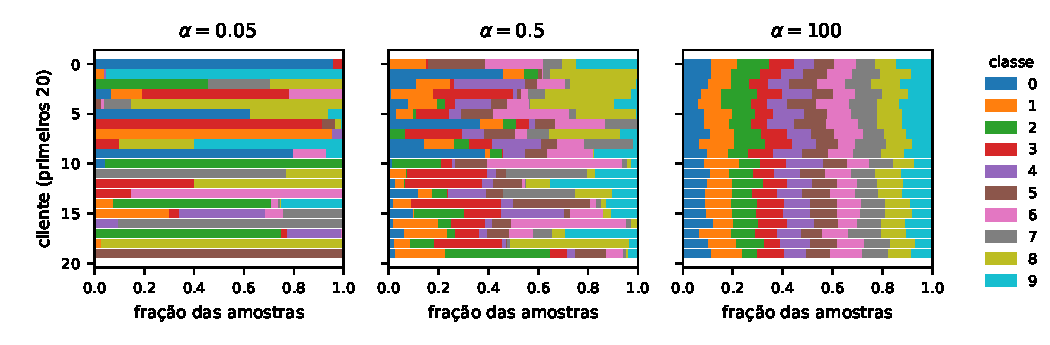
\includegraphics[width=0.92\textwidth]{figs/particoes.pdf}
    \caption{Distribuição de rótulos nos 20 primeiros de 100 clientes, na partição de Dirichlet por classe, para três valores de $\alpha$, em um conjunto balanceado de 10 classes com 5.000 amostras cada (como o CIFAR-10). Cada barra é um cliente, e as cores indicam a fração de cada classe. Com $\alpha = 0{,}05$, a maioria dos clientes vê uma ou duas classes; com $\alpha = 100$, as proporções são praticamente uniformes. Gerada por \texttt{scripts/fig\_particoes.py}.}
    \label{fig:dirichlet}
\end{figure*}

\subsubsection{Por que dados não-IID degradam o FedAvg: o \textit{client drift}}

\citet{zhao2018noniid} quantificaram o efeito empiricamente. Em partições em que cada cliente tem uma única classe, a acurácia do FedAvg caiu até cerca de 11\% no MNIST e 51\% no CIFAR-10 em relação ao SGD centralizado com lotes de mesmo tamanho. Os autores atribuem a queda à \emph{divergência dos pesos}: a distância entre o modelo federado e um modelo treinado de forma centralizada cresce com a distância entre a distribuição de classes de cada cliente e a da população.

O mecanismo por trás dessa divergência é o \textit{client drift}. Quando $P_k \neq P$, o minimizador de $F_k$ não coincide com o de $F$. Cada passo local aproxima $w_k$ do ótimo local, e quanto mais passos ($E$ maior), mais o modelo local se afasta da direção que reduziria $F$. A média da Equação~\eqref{eq:fedavg} combina modelos que foram puxados para lados diferentes e, por isso, não corresponde a um passo de descida em $F$. \citet{karimireddy2020scaffold} mostram que esse efeito existe mesmo com participação total e gradientes exatos, ou seja, não decorre apenas do ruído da amostragem de clientes.

Os resultados de convergência expressam o fenômeno por meio de medidas de \emph{dissimilaridade} entre clientes. \citet{li2020convergence} provam que, para funções fortemente convexas e suaves, o FedAvg converge sob dados não-IID a uma taxa $O(1/T)$, mas a constante cresce com $\Gamma = F^\ast - \sum_k \frac{n_k}{n} F_k^\ast$, que mede o quanto os ótimos locais diferem do global; mostram ainda que, com taxa de aprendizado fixa e $E > 1$, o FedAvg converge para um ponto afastado do ótimo. \citet{li2020fedprox} usam outra medida, a dissimilaridade $B$-local, definida por $\mathbb{E}_k \lVert \nabla F_k(w)\rVert^2 \leq B^2 \lVert \nabla F(w)\rVert^2$: com dados IID, $B \to 1$, e quanto mais heterogêneos os clientes, maior $B$. Embora as medidas difiram, a conclusão é comum: a heterogeneidade impõe um compromisso entre fazer mais trabalho local, para economizar comunicação, e fazer menos, para limitar a deriva.

\subsubsection{Heterogeneidade de sistema}

A heterogeneidade estatística se soma à \emph{heterogeneidade de sistema}: diferenças de processamento, memória, bateria e conectividade entre dispositivos \citep{li2020challenges, lim2020mobileedge}. Na prática, clientes lentos (\textit{stragglers}) não completam as $E$ épocas no prazo da rodada. Na implementação usual do FedAvg, esses clientes são descartados \citep{li2020fedprox}, o que, sob dados não-IID, retira sistematicamente da agregação a contribuição de certas partes da distribuição. Os dois tipos de heterogeneidade interagem, e parte dos algoritmos discutidos a seguir foi desenhada para lidar com ambos.

% ============================================================
\subsection{Abordagens, métodos e soluções existentes}
\label{ref:abordagens}

As propostas para mitigar o \textit{client drift} podem ser agrupadas pelo ponto em que atuam: no problema que o cliente resolve, na forma como as atualizações são combinadas ou no otimizador do servidor. A distinção é relevante na borda, porque determina \emph{quem paga o custo} da correção: o cliente, que é o nó mais restrito, ou o servidor.

\subsubsection{Correção no cliente: FedProx}

O FedProx \citep{li2020fedprox} altera apenas o problema resolvido localmente. Em vez de minimizar $F_k(w)$, o cliente minimiza
\begin{equation}
    h_k(w; w^t) = F_k(w) + \frac{\mu}{2}\lVert w - w^t \rVert^2 ,
    \label{eq:fedprox}
\end{equation}
cujo gradiente é $\nabla F_k(w) + \mu (w - w^t)$. O termo proximal age como uma mola que puxa o modelo local de volta ao global e limita o quanto ele pode derivar, mesmo quando o número de passos locais é grande. O hiperparâmetro $\mu$ controla a rigidez dessa mola: com $\mu = 0$ o FedProx coincide com o FedAvg, e com $\mu$ grande o cliente quase não sai de $w^t$, o que estabiliza o treinamento, mas o torna lento.

A segunda ideia do FedProx é aceitar soluções \emph{$\gamma$-inexatas} do problema local: cada cliente pode executar uma quantidade variável de trabalho, desde que reduza o gradiente de $h_k$ por um fator $\gamma$. Isso permite incorporar o trabalho parcial de \textit{stragglers} em vez de descartá-lo. A análise de convergência, que cobre também o caso não convexo, relaciona $\gamma$, $\mu$ e a dissimilaridade $B$, e as condições para garantir progresso ficam mais restritivas à medida que $B$ cresce. Nos experimentos originais, a maior vantagem sobre o FedAvg (em média 22 pontos percentuais de acurácia) apareceu no cenário com 90\% de \textit{stragglers}, que o FedAvg descarta; sem \textit{stragglers}, o ganho existe, mas é menor. Por isso, resultados obtidos só com heterogeneidade estatística não devem ser comparados diretamente aos números do artigo original.

Do ponto de vista de custo, a agregação do FedProx é a mesma da Equação~\eqref{eq:fedavg}, e o volume transmitido por rodada é idêntico ao do FedAvg. O custo adicional é inteiramente local: manter uma cópia de $w^t$ na memória e calcular o termo e seu gradiente a cada passo, uma operação $O(d)$ no número $d$ de parâmetros. Em termos assintóticos, esse custo é pequeno diante da retropropagação, que também é $O(d)$ por amostra, mas é multiplicada pelo tamanho do lote. Na prática, porém, o NIID-Bench \citep{li2022niidbench} mediu tempos por rodada do FedProx de 15\% a quase 200\% maiores que os do FedAvg (por exemplo, 193~s contra 233~s no CIFAR-10 e 73~s contra 133~s no MNIST), atribuindo a diferença ao cálculo do termo proximal em cada lote. A distância entre a estimativa assintótica e a medição indica que o custo depende da implementação e do hardware, e os autores não descrevem o hardware usado, de modo que não se sabe quanto esse custo representa em um dispositivo restrito.

\subsubsection{Correção no cliente e na agregação: SCAFFOLD e FedNova}

O \textbf{SCAFFOLD} \citep{karimireddy2020scaffold} corrige a direção do gradiente em vez de penalizar a distância. O servidor mantém uma variável de controle global $c$, e cada cliente mantém uma variável local $c_k$; $c$ estima a direção de atualização do servidor e $c_k$, a do cliente $k$, de modo que $c - c_k$ estima a deriva do cliente. O passo local usa $\nabla F_k(w) - c_k + c$, o que compensa essa deriva. Os autores provam que a convergência do SCAFFOLD não depende da dissimilaridade entre clientes. O custo é dobrar o volume transmitido (modelo e variável de controle) e exigir que o cliente guarde $c_k$ entre rodadas. Os autores relatam que o método é relativamente robusto à amostragem de clientes, mas, quando cada cliente participa raramente, como no cenário \textit{cross-device}, $c_k$ fica desatualizado e manter estado no cliente é, por si só, uma restrição \citep{kairouz2021advances}.

O \textbf{FedNova} \citep{wang2020fednova} trata outro aspecto do problema. Quando os clientes executam números diferentes de passos locais $\tau_k$, por terem mais dados ou mais poder computacional, o FedAvg passa a otimizar implicitamente uma função objetivo ponderada por $n_k \tau_k$, diferente da Equação~\eqref{eq:objetivo}; os autores chamam isso de \emph{inconsistência de objetivo}. O FedNova atua na agregação: normaliza cada atualização por $\tau_k$ antes da média, sem custo extra relevante no cliente. Esse problema é particularmente relevante sob desvio de quantidade com número fixo de épocas, em que $\tau_k$ é proporcional a $n_k$.

\subsubsection{Correção no servidor: FedAvgM e FedAdam}

Uma linha alternativa mantém o cliente igual ao FedAvg e muda apenas o servidor. A observação comum é que a diferença entre o modelo global e a média dos modelos locais, $\Delta^t = w^t - \sum_{k \in S_t} \frac{n_k}{\sum_{j\in S_t} n_j} w_k^{t+1}$, pode ser tratada como um \emph{pseudo-gradiente} e alimentar qualquer otimizador. O \textbf{FedAvgM} \citep{hsu2019fedavgm} aplica momento ao pseudo-gradiente, o que suaviza as oscilações entre rodadas causadas por clientes que puxam em direções diferentes. Foi também nesse trabalho que a partição de Dirichlet passou a ser usada para varrer o nível de heterogeneidade, e os autores mostraram que a acurácia do FedAvg cai de forma contínua à medida que $\alpha$ diminui. \citet{reddi2021adaptive} generalizam a ideia no arcabouço FedOpt, com otimizadores adaptativos no servidor (\textbf{FedAdam}, FedYogi, FedAdagrad), e relatam ganhos consistentes sobre o FedAvg em tarefas com heterogeneidade natural.

Essas abordagens não exigem estado nem computação adicional no cliente e não alteram o volume transmitido. Na borda, onde o servidor é o nó com mais recursos, isso as torna contrapontos naturais ao FedProx: se oferecem ganho semelhante sem custo para o dispositivo, o argumento a favor do FedProx enfraquece. A desvantagem é acrescentar hiperparâmetros no servidor (taxa de aprendizado global, momento), aos quais o desempenho é sensível.

\subsubsection{Comparação entre as abordagens}

A Tabela~\ref{tab:abordagens} resume as diferenças. Duas observações orientam a escolha dos algoritmos deste trabalho. Primeiro, apenas FedProx e SCAFFOLD alteram o cálculo feito no cliente e, portanto, são os únicos cujo custo local pode diferir do FedAvg. Segundo, cada algoritmo tem um hiperparâmetro próprio cuja escolha condiciona o resultado ($\mu$, momento, taxa do servidor), de modo que uma comparação justa precisa variar ou ao menos calibrar esses valores.

\begin{table*}[t]
    \centering\small
    \caption{Comparação conceitual entre as abordagens de mitigação do \textit{client drift}. Custos relativos ao FedAvg; $d$ = número de parâmetros do modelo.}
    \label{tab:abordagens}
    \setlength{\tabcolsep}{4pt}
    \begin{tabular}{@{}>{\raggedright\arraybackslash}p{2.9cm}>{\raggedright\arraybackslash}p{1.4cm}>{\raggedright\arraybackslash}p{4.6cm}>{\raggedright\arraybackslash}p{1.6cm}>{\raggedright\arraybackslash}p{2.7cm}>{\raggedright\arraybackslash}p{1.2cm}>{\raggedright\arraybackslash}p{1.9cm}@{}}
        \toprule
        Algoritmo & Onde atua & Mecanismo & Comunic. & Custo no cliente & Estado & Hiperparâm. \\
        \midrule
        FedAvg\newline \citep{mcmahan2017fedavg} & -- & Média ponderada de modelos locais & $1\times$ & -- & Não & $E$, taxa local \\
        FedProx\newline \citep{li2020fedprox} & Cliente & Termo proximal limita a distância a $w^t$; aceita trabalho parcial & $1\times$ & $+O(d)$ por passo; cópia de $w^t$ & Não & $\mu$ \\
        SCAFFOLD\newline \citep{karimireddy2020scaffold} & Cliente & Variáveis de controle corrigem a direção do gradiente & $2\times$ & $+O(d)$ por passo; cópia de $c$, $c_k$ & Sim ($c_k$) & -- \\
        FedNova\newline \citep{wang2020fednova} & Agregação & Normaliza atualizações pelo número de passos locais & $\approx 1\times$ & desprezível & Não & -- \\
        FedAvgM\newline \citep{hsu2019fedavgm} & Servidor & Momento sobre o pseudo-gradiente & $1\times$ & -- & Não & momento $\beta$ \\
        FedAdam\newline \citep{reddi2021adaptive} & Servidor & Adam sobre o pseudo-gradiente & $1\times$ & -- & Não & taxa global, adaptatividade \\
        \bottomrule
    \end{tabular}
\end{table*}

\subsubsection{Evidência empírica e lacunas da literatura}

A teoria indica \emph{por que} cada algoritmo deveria funcionar, mas sob hipóteses (suavidade, dissimilaridade ou gradientes limitados) difíceis de verificar em redes profundas, e com constantes que não permitem prever a magnitude do ganho. A questão prática, quanto cada um ganha em cenários concretos, é respondida por estudos comparativos, analisados em detalhe na Seção~\ref{trabalhosrelacionados}. Para a fundamentação, importam três constatações.

\textbf{Os resultados divergem.} O NIID-Bench \citep{li2022niidbench} conclui que nenhum algoritmo é sempre o melhor. O FedProx costuma obter a melhor acurácia sob desvio de rótulos e de quantidade, mas o melhor $\mu$ na grade $\{0{,}001; 0{,}01; 0{,}1; 1\}$ foi sempre pequeno, e nesses casos os dois algoritmos têm convergência e acurácia semelhantes. Estudos de aplicação relatam tanto a superioridade do FedProx \citep{mahmood2025alzheimer, delehouzee2024crosssilo, julekha2026bangla} quanto resultados em que ele não supera o FedAvg \citep{vajjhula2025har, quintana2026mammography}. Sem conhecer o $\mu$ usado, não se sabe se um resultado negativo indica que o FedProx não funciona ou que $\mu$ foi mal escolhido.

\textbf{O efeito depende do tipo de desvio e do nível.} O NIID-Bench observa que o caso com uma única classe por cliente é o mais difícil e que os desvios de atributos e de quantidade têm pouca influência na acurácia do FedAvg. Muitos estudos, porém, comparam apenas ``IID × não-IID''. A dependência contínua da acurácia em $\alpha$, mostrada por \citet{hsu2019fedavgm} para o FedAvg, não foi encontrada para a \emph{diferença} entre FedProx e FedAvg nos estudos analisados.

\textbf{O custo local é medido de forma incompleta.} Os estudos priorizam métricas de qualidade e, quando medem custo, em geral medem comunicação \citep{bakr2026parkfl, tan2026instruction}, item em que FedAvg e FedProx são idênticos por construção. O \textit{overhead} medido pelo NIID-Bench, em hardware não descrito, é muito maior do que a análise assintótica sugere, o que indica forte dependência da implementação. Nas fontes consultadas, ela não foi repetida em dispositivo restrito nem combinada ao número de rodadas economizadas. Além disso, quase todos os resultados vêm de simulação, e \citet{valli2026beyond} alertam que conclusões obtidas em simulação nem sempre se mantêm em implantações reais.

\subsubsection{Ferramentas para simulação federada}

A reprodutibilidade dos estudos depende das ferramentas. O \textbf{Flower} \citep{beutel2020flower} é um framework de código aberto para FL, agnóstico à biblioteca de aprendizado, que oferece implementações prontas de FedAvg, FedProx, FedAvgM e FedAdam, um motor de simulação apoiado no Ray \citep{moritz2018ray} capaz de executar centenas de clientes virtuais em uma máquina e a mesma API para implantação em dispositivos reais. A biblioteca \textbf{Flower Datasets} implementa os particionadores discutidos acima (Dirichlet por classe, patológico, por tamanho). Os modelos e o treinamento local são implementados em \textbf{PyTorch} \citep{paszke2019pytorch}. Para comparar algoritmos, benchmarks como LEAF \citep{caldas2018leaf} oferecem datasets com heterogeneidade natural, enquanto CIFAR-10 \citep{krizhevsky2009cifar} e Fashion-MNIST \citep{xiao2017fashion} são opções comuns com partições sintéticas.

% ============================================================
\subsection{Síntese e relação com a pesquisa proposta}
\label{ref:sintese}

O referencial estabelece uma cadeia de argumentos que leva diretamente ao problema deste trabalho. O FedAvg economiza comunicação fazendo vários passos locais, mas, sob dados não-IID, esses passos derivam para os ótimos locais, e a teoria mostra que o prejuízo cresce com a dissimilaridade entre clientes. O FedProx ataca essa deriva no próprio cliente, com um termo cujo efeito depende de $\mu$ e cujo custo recai sobre o dispositivo. Alternativas como FedAvgM e FedAdam atacam o mesmo problema no servidor, sem custo para o cliente, e o SCAFFOLD corrige a direção do gradiente ao preço de comunicação e estado extras. A evidência empírica, porém, não permite dizer quando a abordagem do FedProx vale a pena.

\paragraph{Conceitos que fundamentam a pesquisa.} Três conceitos são centrais: o \textit{client drift}, que explica por que a heterogeneidade prejudica o FedAvg e por que o termo proximal deveria ajudar; a partição de Dirichlet e seu parâmetro $\alpha$, que tornam o nível de heterogeneidade uma variável contínua e controlável; e a distinção entre tipos de desvio, que mostra que ``não-IID'' não é uma condição única.

\paragraph{Abordagens mais relevantes.} A comparação central é FedProx × FedAvg, já que o segundo é o caso $\mu = 0$ do primeiro, o que permite isolar o efeito do termo proximal. SCAFFOLD, FedAvgM e FedAdam entram como referências. O SCAFFOLD representa a outra forma de correção no cliente, com custo de comunicação e de estado, e FedAvgM e FedAdam, a correção no servidor, sem custo no cliente; juntos, indicam se o ganho do FedProx é grande ou pequeno diante das alternativas. O FedNova, que corrige a agregação, não entra na grade principal por limite de orçamento computacional, e não por irrelevância: na partição de Dirichlet por classe os tamanhos $n_k$ variam e, com épocas fixas, $\tau_k$ também varia, o que gera a inconsistência de objetivo que ele corrige. Ele fica como primeira extensão, prioritariamente no cenário de desvio de quantidade.

\paragraph{Decisões orientadas pela literatura.} Cada lacuna corresponde a uma decisão de desenho:
\begin{itemize}[leftmargin=*, itemsep=1pt]
    \item Contra a contradição dos resultados, $\mu$ será tratado como variável ($\mu \in \{0{,}01; 0{,}1; 1\}$), incluindo valores pequenos, que o NIID-Bench identificou como ótimos, e um valor alto; $\mu = 0{,}001$ fica de fora, por se aproximar de $\mu = 0$, que é o próprio FedAvg. Cada configuração será executada com várias sementes pareadas, como em \citet{enang2026optimiser}, com teste de Wilcoxon \citep{wilcoxon1945} para diferenças e teste de equivalência \citep{schuirmann1987tost} para afirmar ausência de diferença.
    \item Para verificar se existe um limiar de heterogeneidade e, se existir, localizá-lo, $\alpha$ varrerá cinco valores, de $0{,}05$ a $100$, seguindo a abordagem de \citet{hsu2019fedavgm}, mas medindo a diferença entre os algoritmos.
    \item Para separar os tipos de desvio, a partição de Dirichlet por classe será comparada à partição patológica (só rótulos) e a uma partição com desvio só de quantidade e rótulos IID, o que resolve a confusão apontada na Seção~\ref{ref:conceitos}.
    \item Para medir o custo local, o tempo por época e a memória de pico serão medidos em CPU restrita a um núcleo, isolando o termo proximal (mesmo código, com e sem o termo), o que permite verificar se o \textit{overhead} relatado pelo NIID-Bench é intrínseco ou de implementação; o custo total até a acurácia-alvo combinará esse tempo com o número de rodadas, refletindo o compromisso descrito por \citet{wang2019adaptive}.
    \item Os experimentos usarão Flower, Flower Datasets e PyTorch, sobre CIFAR-10, um dos datasets mais usados pelos estudos comparados, e Fashion-MNIST, mais barato e também usado no NIID-Bench, o que facilita contrastar os resultados.
\end{itemize}

\paragraph{Refinamento dos objetivos.} A análise da literatura confirmou o problema e os objetivos apresentados na Introdução e levou a dois ajustes de escopo. Primeiro, o desvio de atributos, previsto inicialmente com o FEMNIST \citep{caldas2018leaf}, ficou fora das hipóteses, porque mistura o tipo de desvio com outras diferenças do dataset e dificultaria isolar o efeito do FedProx. Segundo, a heterogeneidade de sistema, cenário original do FedProx, foi mantida apenas como extensão, para que a comparação principal trate somente da heterogeneidade estatística, que é onde a literatura diverge. As próximas etapas do trabalho são formalizar as hipóteses derivadas dessas lacunas, construir o ambiente de simulação e executar o projeto fatorial resumido na Introdução.
